% version 1.00, date 20/02/16, auteur Michel Cressant
\begin{figure}[H]
\centering 
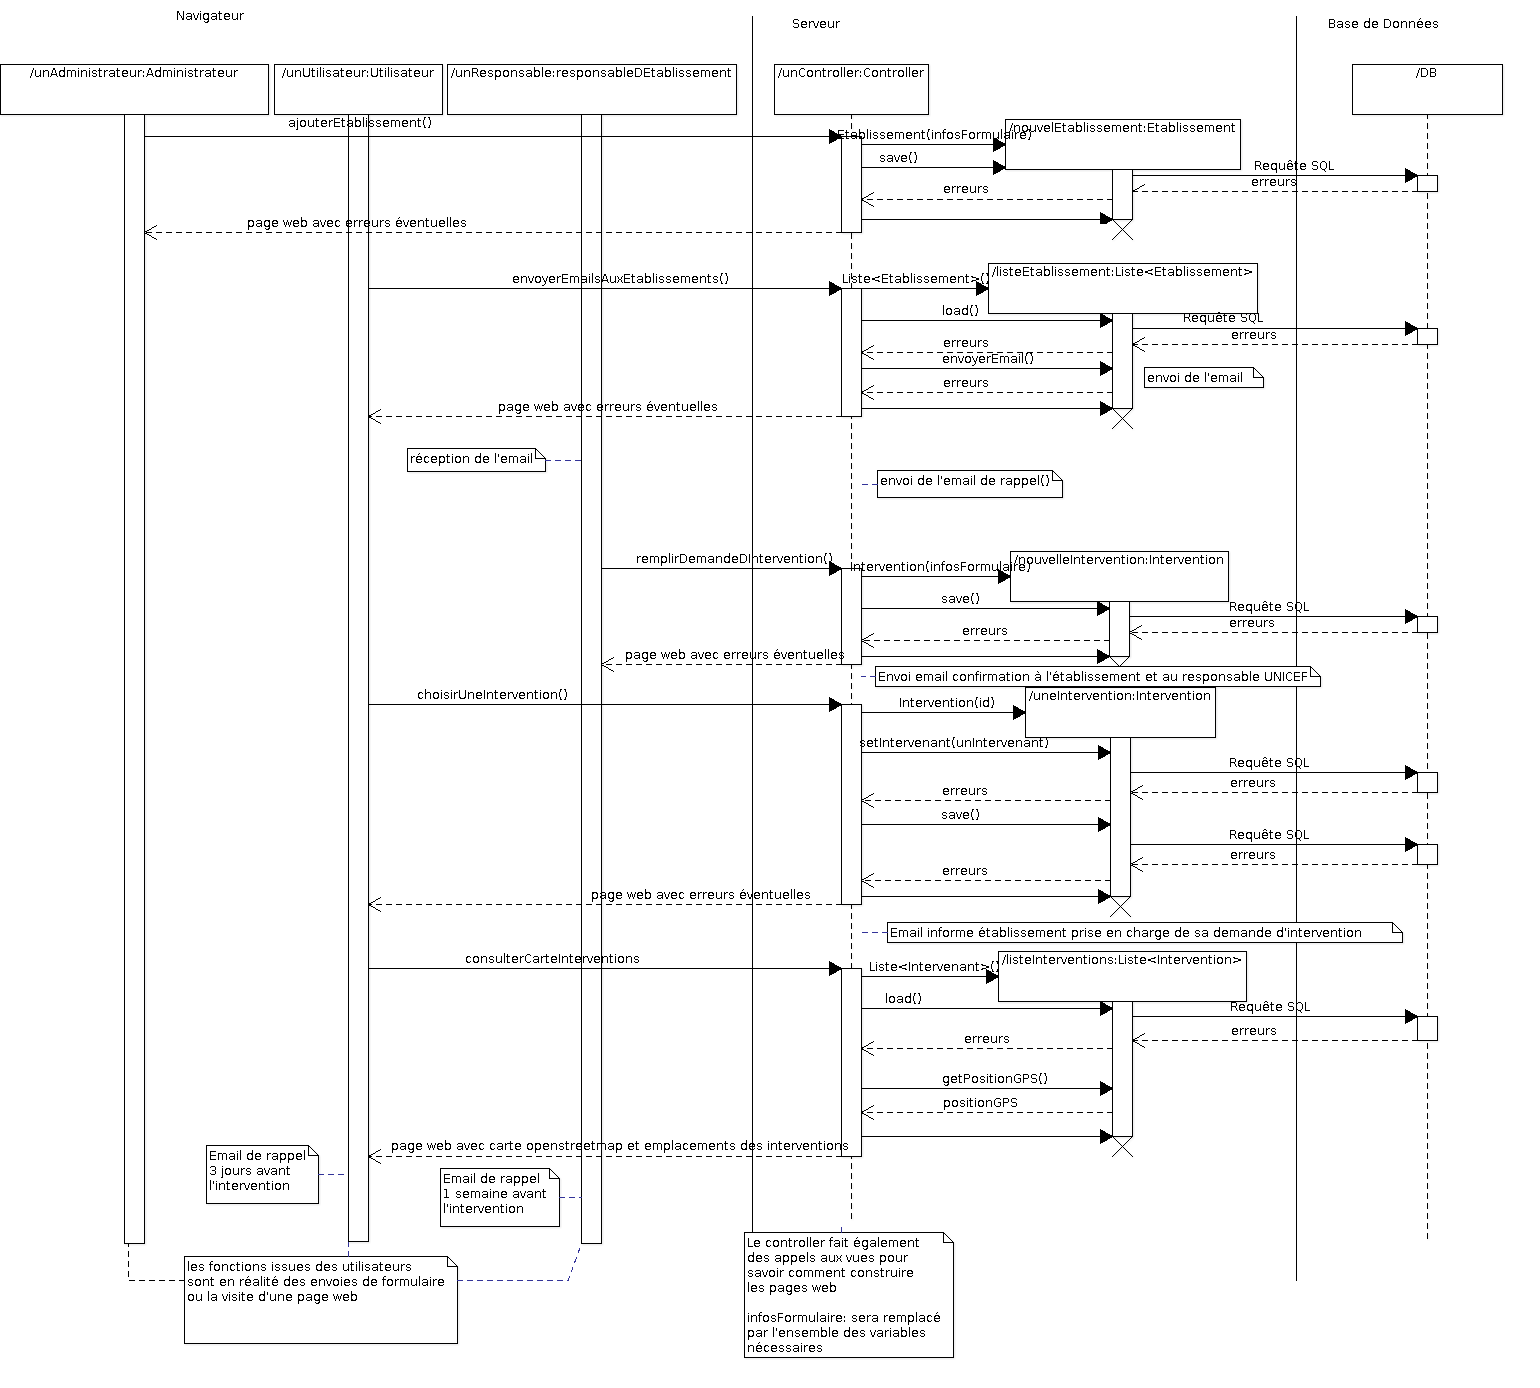
\includegraphics[scale=0.34]{images/diagrammeSequenceSysteme/diagrammeSequence.png}
\caption{Diagramme de séquence système}
\label{diagrammeDeSequenceSysteme}
\end{figure}

Ce diagramme (figure \ref{diagrammeDeSequenceSysteme}) présente le diagramme de séquence système du lot 2 de notre projet. \\
Comme présenté sur la figure, l'administrateur pourra ajouter un établissement à la base de données. Cette dernière action peut se décomposer en plusieurs étapes : 
\begin{itemize}
	\item l'administrateur clique sur ajouter un établissement;
	\item l'administrateur entre les données de l'établissement dans le formulaire;
	\item le contrôleur récupère les informations du formulaire et met à jour la base de données;
	\item si une erreur apparaît, une page d'erreur est renvoyée à l'administrateur.\\
\end{itemize}


La création de profil s'effectuera de la même manière que l'ajout d'un établissement à la base de données, seules les informations demandées dans les formulaires diffèreront.\\



Une autre des fonctionnalités de notre lot 2 est l'envoi d'e-mails aux établissements. Celle-ci peut également se décomposer en diférentes étapes : 
\begin{itemize}
	\item l'utilisateur déclenche l'envoi d'e-mails aux établissements; 
	\item le contrôleur récupère la liste des adresses e-mails des établissements;
	\item le contôleur envoie à cette liste d'adresses un e-mails un courriel type afin de proposer aux établissements des interventions pour sensibiliser les enfants à différents thèmes. Cet e-mail contiendra un lien vers un formulaire qui permettra aux établissements d'effectuer des demandes d'intervention;
	\item si une erreur se produit, une page d'erreur sera renvoyée à l'utilisateur;
	\item si l'établissement ne remplit le formulaire de demande d'interventions après un certain temps, un e-mail de rappel sera envoyé aux établissements. \\
\end{itemize}   


L'étape suivante est le remplissage du formulaire par l'établissement demandeur. A chaque demande d'interventions:  
\begin{itemize}
	\item chaque intervention de la demande de l'établissement sera ajouté à la base de données;
	\item un e-mail de confirmation de demande d'interventions sera envoyé à l'établissement, lui permettant également d'annuler cette dernière;
	\item un e-mail d'information sera envoyé aux responsables d'activitéde l'UNICEF;
	\item en cas d'erreur, une page d'erreur sera renvoyée à l'utilisateur.\\
\end{itemize}


Lorsque la base de données contiendra des interventions, un bénévole pourra choisir une intervention et se l'attribuer. Cette action donnera une valeur à l'intervenant de l'intervention dans la base de données. Si une erreur se produit, une page d'erreur sera renvoyée. A chaque attribution d'une intervention à un intervenant, un e-mail d'information de prise en charge de la demande sera envoyé à l'établissement et au reponsable de l'activité de l'UNICEF. \\

Notre produit permettra également de visualiser une carte présentant toutes les interventions pour une date et un moment entrés par l'utilisateur. En cas d'erreur, une page d'erreur sera renvoyée à l'utilisateur. \\

Le plaideur responsable d'une intervention pourra mettre à jour les informations des interventions desquelles il est reponsable. Cela entrainera une mise à jour des interventions modifiées dans la base de données. Après chaque mise à jour, un e-mail informant l'établissement des mises à jour sera envoyée. \\

Une semaine avant chaque intervention, un e-mail sera envoyé à l'établissement concerné.  
Trois jours avant chaque intervention, un e-mail sera envoyé au plaideur responsable de l'intervention. 


